% ==============================================================================
% Section 11: Hedging Efficiency & Terminal Payoff Analytics
% Target: Page 12 (Exactly 1 Page)
% ==============================================================================

\section{Hedging Efficiency and Terminal Payoff Analytics}
\label{sec:payoff_analytics}

\subsection{Terminal Payoff Geometry and Convexity Transformation}

The central goal of derivative engineering is \textbf{payoff transformation}. An unhedged stock holding displays linear exposure to market prices: $V(S_T) = N_{\text{shares}} S_T$, yielding unbounded downside risk. By introducing option overlays, the portfolio's terminal payoff profile is reshaped into non-linear, convex payoff geometries \citep{wilmott2006paul}.

\begin{figure}[!htbp]
    \centering
    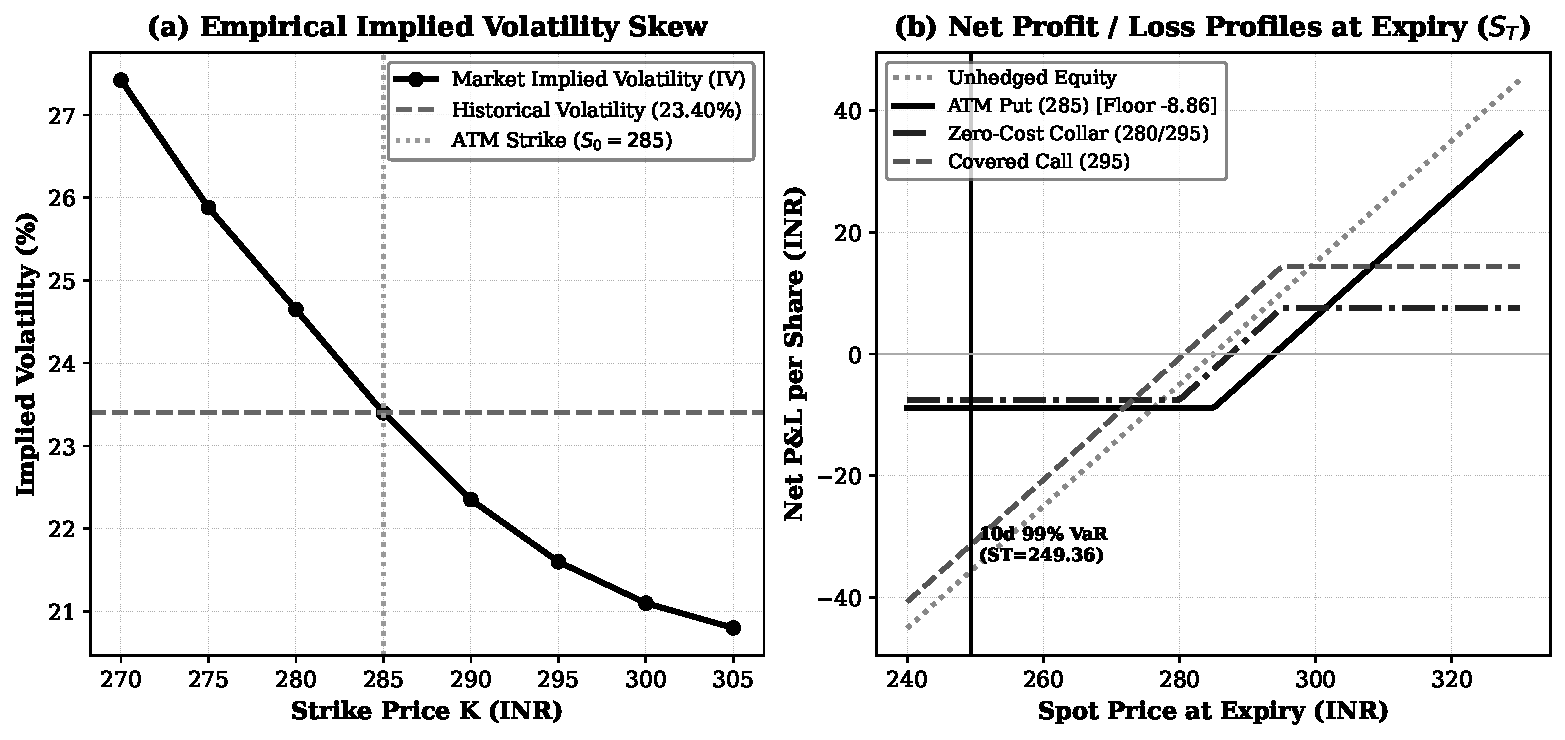
\includegraphics[width=0.96\textwidth, height=6.2cm, keepaspectratio]{figures/fig2_fed_skew_payoffs.pdf}
    \caption{Empirical Implied Volatility Skew and Multi-Strategy Terminal Payoff Profiles for 1 Lot of ITC Limited ($1,725$ Shares, $V_0 = \text{\inr}4,91,625.00$). The upper panel depicts the steep downside IV skew. The lower panels display net terminal P\&L across: (A) ATM Protective Put, (B) OTM Protective Put, (C) Covered Call, and (D) Low-Cost Collar.}
    \label{fig:fed_skew_payoffs}
\end{figure}

\subsection{Comparative Analysis of Payoff Geometries}

Evaluating the terminal payoff profiles illustrated in Figure~\ref{fig:fed_skew_payoffs} reveals distinct risk-return trade-offs:
\begin{itemize}[leftmargin=1.5em, itemsep=1pt, parsep=0pt]
    \item \textbf{Convexity Creation via Protective Puts:} Adding a long put introduces positive Gamma ($\Gamma > 0$), creating an asymmetric profile where portfolio delta expands as prices decline, establishing a hard floor below which losses cannot pass.
    \item \textbf{Asymmetric Premium Drag:} The ATM Put guarantees absolute capital preservation at \inr 285.00, but imposes a drag of \inr 15,283.50 ($3.11\%$) on portfolio return over the 42-day lifespan.
    \item \textbf{Risk Compression via Collars:} The Low-Cost Collar sacrifices extreme upside beyond \inr 295.00 to fund downside insurance below \inr 280.00, compressing return variance into a tightly controlled corridor with net cost of only $0.88\%$.
\end{itemize}

\clearpage
